% !TeX program = xelatex
% !TeX options = -shell-escape
% !TEX encoding = UTF-8

% --------------------------------------------------------------
% This is all preamble stuff that you don't have to worry about.
% Head down to where it says "Start here"
% --------------------------------------------------------------

\documentclass[12pt]{article}
\usepackage[margin=2cm]{geometry} % 頁面邊距設置
\usepackage{amsmath,amssymb,amsthm} % 數學相關套件
\usepackage{graphicx} % 圖形插入
\usepackage{booktabs} % 表格線條
\usepackage[AutoFakeBold,AutoFakeSlant]{xeCJK} % 中文支援
\usepackage{fancyhdr} % 頁首頁尾設置
\usepackage{xcolor,changepage,mdframed} % 顏色與框線相關
\usepackage{titlesec} % 標題格式
\usepackage{setspace} % 行距
\usepackage{minted} % 程式碼高亮（需安裝 Python 套件 pygments）
\usepackage[shortlabels]{enumitem} % 列表格式
\usepackage[colorlinks=true,linkcolor=black,urlcolor=blue,citecolor=blue]{hyperref} % 超連結
\graphicspath{{images}}

% 字體設定 (xeCJK)
\setCJKmainfont{黑體-繁}
\setCJKmonofont{Noto Sans CJK TC}

% 頁首/頁尾設定 (fancyhdr)
\pagestyle{fancy}
\fancyhead[L]{NASA Homework 0} % 可以用 \leftmark 取代
\fancyhead[R]{B13901011 吳亞倫}
\fancyfoot[C]{\thepage}
\renewcommand{\headrulewidth}{0.4pt}
\renewcommand{\footrulewidth}{0pt}
\setlength{\headheight}{15pt}

% tex-fmt: off
\newtheorem*{theorem}{Theorem}
\newenvironment{lemma}[2][Lemma]{\begin{trivlist}
\item[\hskip \labelsep {\bfseries #1}\hskip \labelsep {\bfseries #2.}]}{\end{trivlist}}
\newenvironment{exercise}[2][Exercise]{\begin{trivlist}
\item[\hskip \labelsep {\bfseries #1}\hskip \labelsep {\bfseries #2.}]}{\end{trivlist}}
\newenvironment{problem}[2][Problem]{\begin{trivlist}
\item[\hskip \labelsep {\bfseries #1}\hskip \labelsep {\bfseries #2}]}{\end{trivlist}}
\newenvironment{question}[2][Question]{\begin{trivlist}
\item[\hskip \labelsep {\bfseries #1}\hskip \labelsep {\bfseries #2.}]}{\end{trivlist}}
\newenvironment{corollary}[2][Corollary]{\begin{trivlist}
\item[\hskip \labelsep {\bfseries #1}\hskip \labelsep {\bfseries #2.}]}{\end{trivlist}}
\newenvironment{solution}{\begin{proof}[Solution]}{\end{proof}}
\newenvironment{answer}{\begin{proof}[Ans]}{\end{proof}}

% 樣式設定
\renewcommand\thesubsection{\arabic{subsection}}
\titleformat{\subsection}{\normalfont\large\bfseries}{\thesubsection.}{0.5em}{}

% 自訂框線環境
\newmdenv[
  linewidth=2pt, linecolor=gray, backgroundcolor=gray!10,
  topline=false, bottomline=false, rightline=false,
  skipabove=10pt, skipbelow=10pt, innerleftmargin=10pt,
  innerrightmargin=0pt, innertopmargin=5pt, innerbottommargin=5pt
]{myquote}

\newenvironment{mycolorbox}[1][gray]{
  \renewmdenv[
    linewidth=2pt, linecolor=#1, backgroundcolor=#1!10,
    topline=false, bottomline=false, rightline=false,
    skipabove=10pt, skipbelow=10pt, innerleftmargin=10pt,
    innerrightmargin=0pt, innertopmargin=5pt, innerbottommargin=5pt
  ]{myquote}
  \begin{myquote}
}{\end{myquote}}

\linespread{1.1}
% \usemintedstyle{xcode}
\setminted{breaklines=true, breakanywhere=true, autogobble=true}

% tex-fmt: on
\begin{document}
\thispagestyle{fancy}

%------------------------------------------------------------
%                         Start here
% -----------------------------------------------------------

\begin{center}
  {\large \bfseries Network Administration / System Administration} \\
  \vspace{1em}
  {\Large \bfseries Homework 1} \\
\end{center}

\vspace{2em}

\begin{tabular}{@{}l l}
  \textbf{Student:} & 吳亞倫 \\
  \textbf{ID:} & B13901011  \\
  \textbf{Department:} & 電機工程學系
\end{tabular}
\bigskip

\subsection{Discussion}
\begin{itemize}
  \item 這次作業我和\,\textbf{賴泓安}、\textbf{鄭竣陽}\,以及\,\textbf{喻慈恩}\,討論。
\end{itemize}

\subsection{Reference}

\begin{problem}{1.} \textbf{參數檢查}
  \begin{itemize}
    \item \href{https://stackoverflow.com/questions/3005963/how-can-i-have-a-newline-in-a-string-in-sh}{How can I have a newline in a string in sh? (Stack Overflow)}
    \item \href{https://stackoverflow.com/questions/17420994/how-can-i-match-a-string-with-a-regex-in-bash}{How can I match a string with a regex in Bash? (Stack Overflow)}
    \item \href{https://zh.wikipedia.org/zh-tw/正则表达式}{正規表達式 - wikipedia}
    \item \href{https://stackoverflow.com/questions/35919103/how-do-i-use-a-regex-in-a-shell-script}{How do I use a regex in a shell script? (Stack Overflow)}
    \item \href{https://hsuchihting.github.io/regex/20220731/4121487144/}{Regular Expression 正則表達式初探 (TimCodingBlog)}
    \item \href{https://ss64.com/bash/test.html}{test man page}
  \end{itemize}
\end{problem}

\begin{problem}{2.} \textbf{Building a Merkle Tree}
  \begin{itemize}
    \item \href{https://stackoverflow.com/questions/23356779/how-can-i-store-the-find-command-results-as-an-array-in-bash/54561526#54561526/}{How can I store the "find" command results as an array in Bash (Stack Overflow)}
    \item \href{https://stackoverflow.com/questions/1951506/add-a-new-element-to-an-array-without-specifying-the-index-in-bash}{Add a new element to an array without specifying the index in Bash (Stack Overflow)}
    \item \href{https://stackoverflow.com/questions/8880603/loop-through-an-array-of-strings-in-bash}{Loop through an array of strings in Bash? (Stack Overflow)}
    \item \href{https://stackoverflow.com/questions/2564634/convert-absolute-path-into-relative-path-given-a-current-directory-using-bash}{Convert absolute path into relative path given a current directory using Bash (Stack Overflow)}
    \item \href{https://ss64.com/bash/test.html}{test man page}
  \end{itemize}
\end{problem}
\begin{problem}{3.} \textbf{Generating an Inclusion Proof}
  \begin{itemize}
    \item \href{https://sysxplore.com/bash-bitwise-operators/#bitwise-xor}{Bash bitwise operators - xor (Sysxplore)}
  \end{itemize}
\end{problem}
\begin{problem}{4.} \textbf{Verifying an Inclusion Proof}
  \begin{itemize}
    \item \href{https://stackoverflow.com/questions/12204192/using-multiple-delimiters-in-awk}{Using multiple delimiters in awk (Stack Overflow)}
    \item \href{https://sysxplore.com/bash-bitwise-operators/#bitwise-and}{Bash bitwise operators - and (Sysxplore)}
    \item \href{https://stackoverflow.com/questions/2264428/how-to-convert-a-string-to-lower-case-in-bash}{How to convert a string to lower case in Bash (Stack Overflow)}
  \end{itemize}
\end{problem}

\subsection{AI conversation}
\begin{problem}{1.} \textbf{參數檢查}
  \begin{figure}[H]
    \centering
    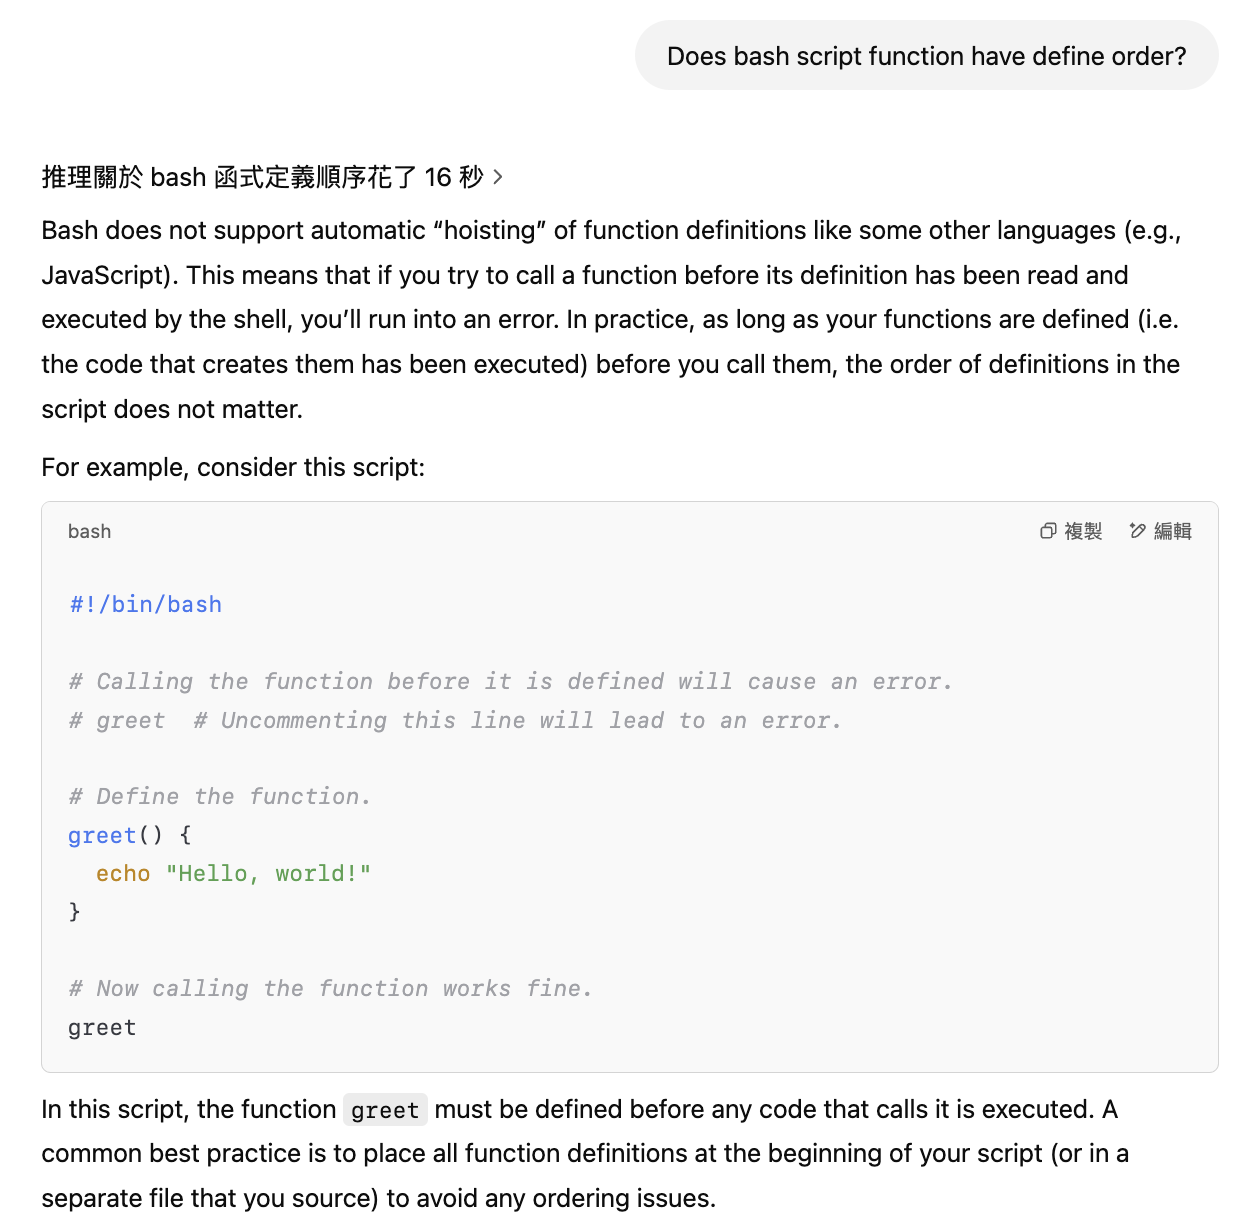
\includegraphics[width=\textwidth]{1-1.png}
  \end{figure}
\end{problem}

\begin{problem}{2.} \textbf{Building a Merkle Tree}
  \begin{itemize}
    \item 本題我沒有使用 chatGPT 輔助
  \end{itemize}
\end{problem}

\clearpage
\begin{problem}{3.} \textbf{Generating an Inclusion Proof}
  \begin{figure}[H]
    \centering
    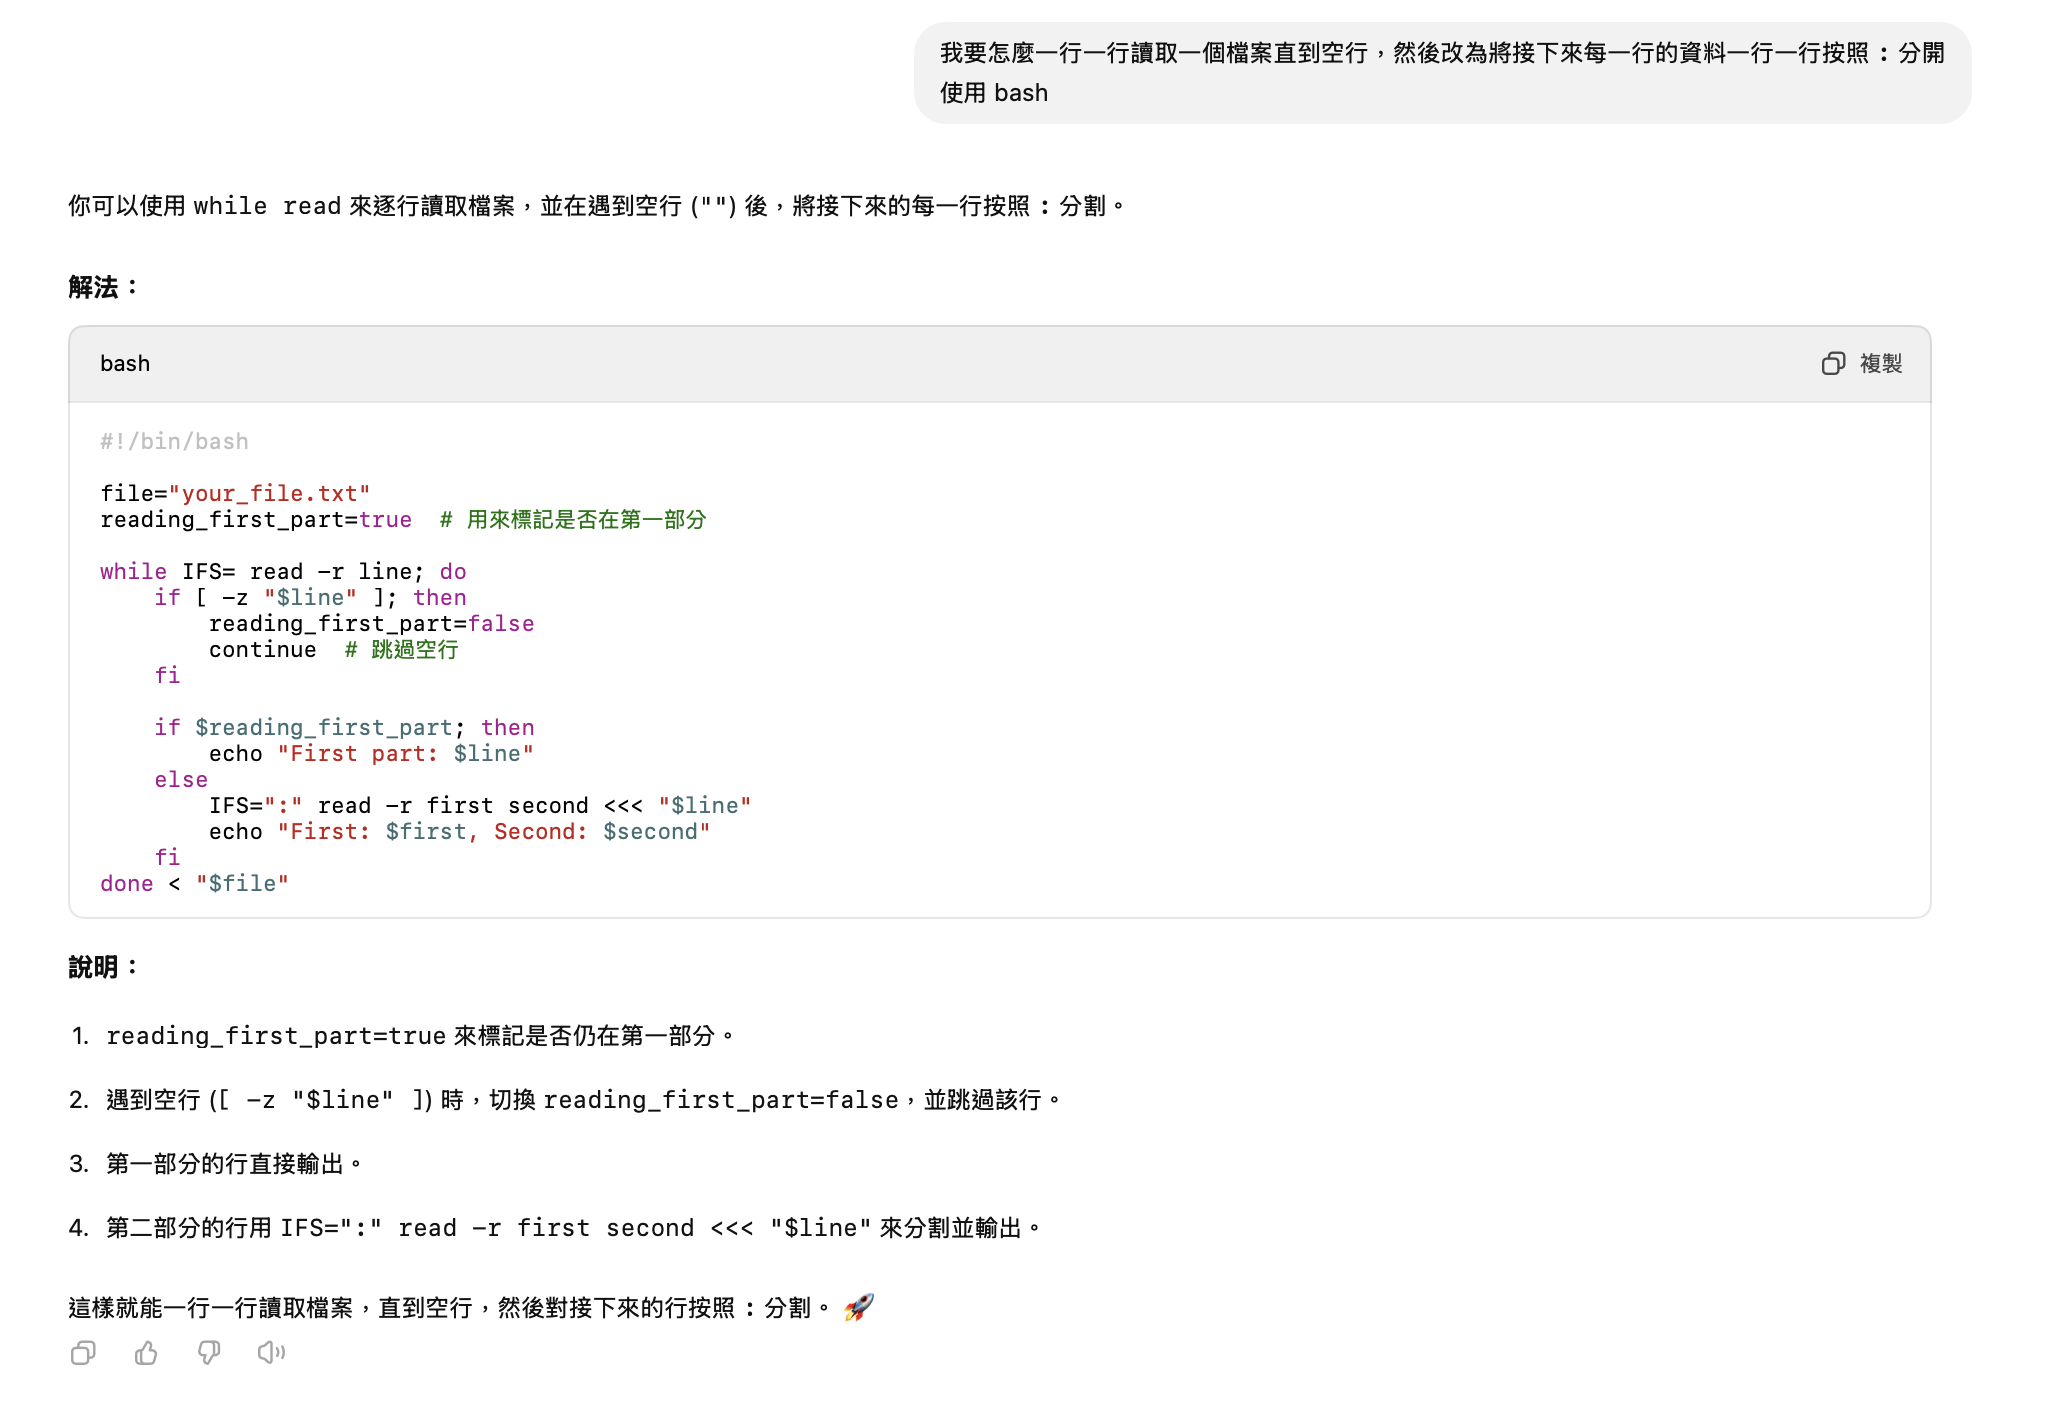
\includegraphics[width=\textwidth]{3-1.png}
    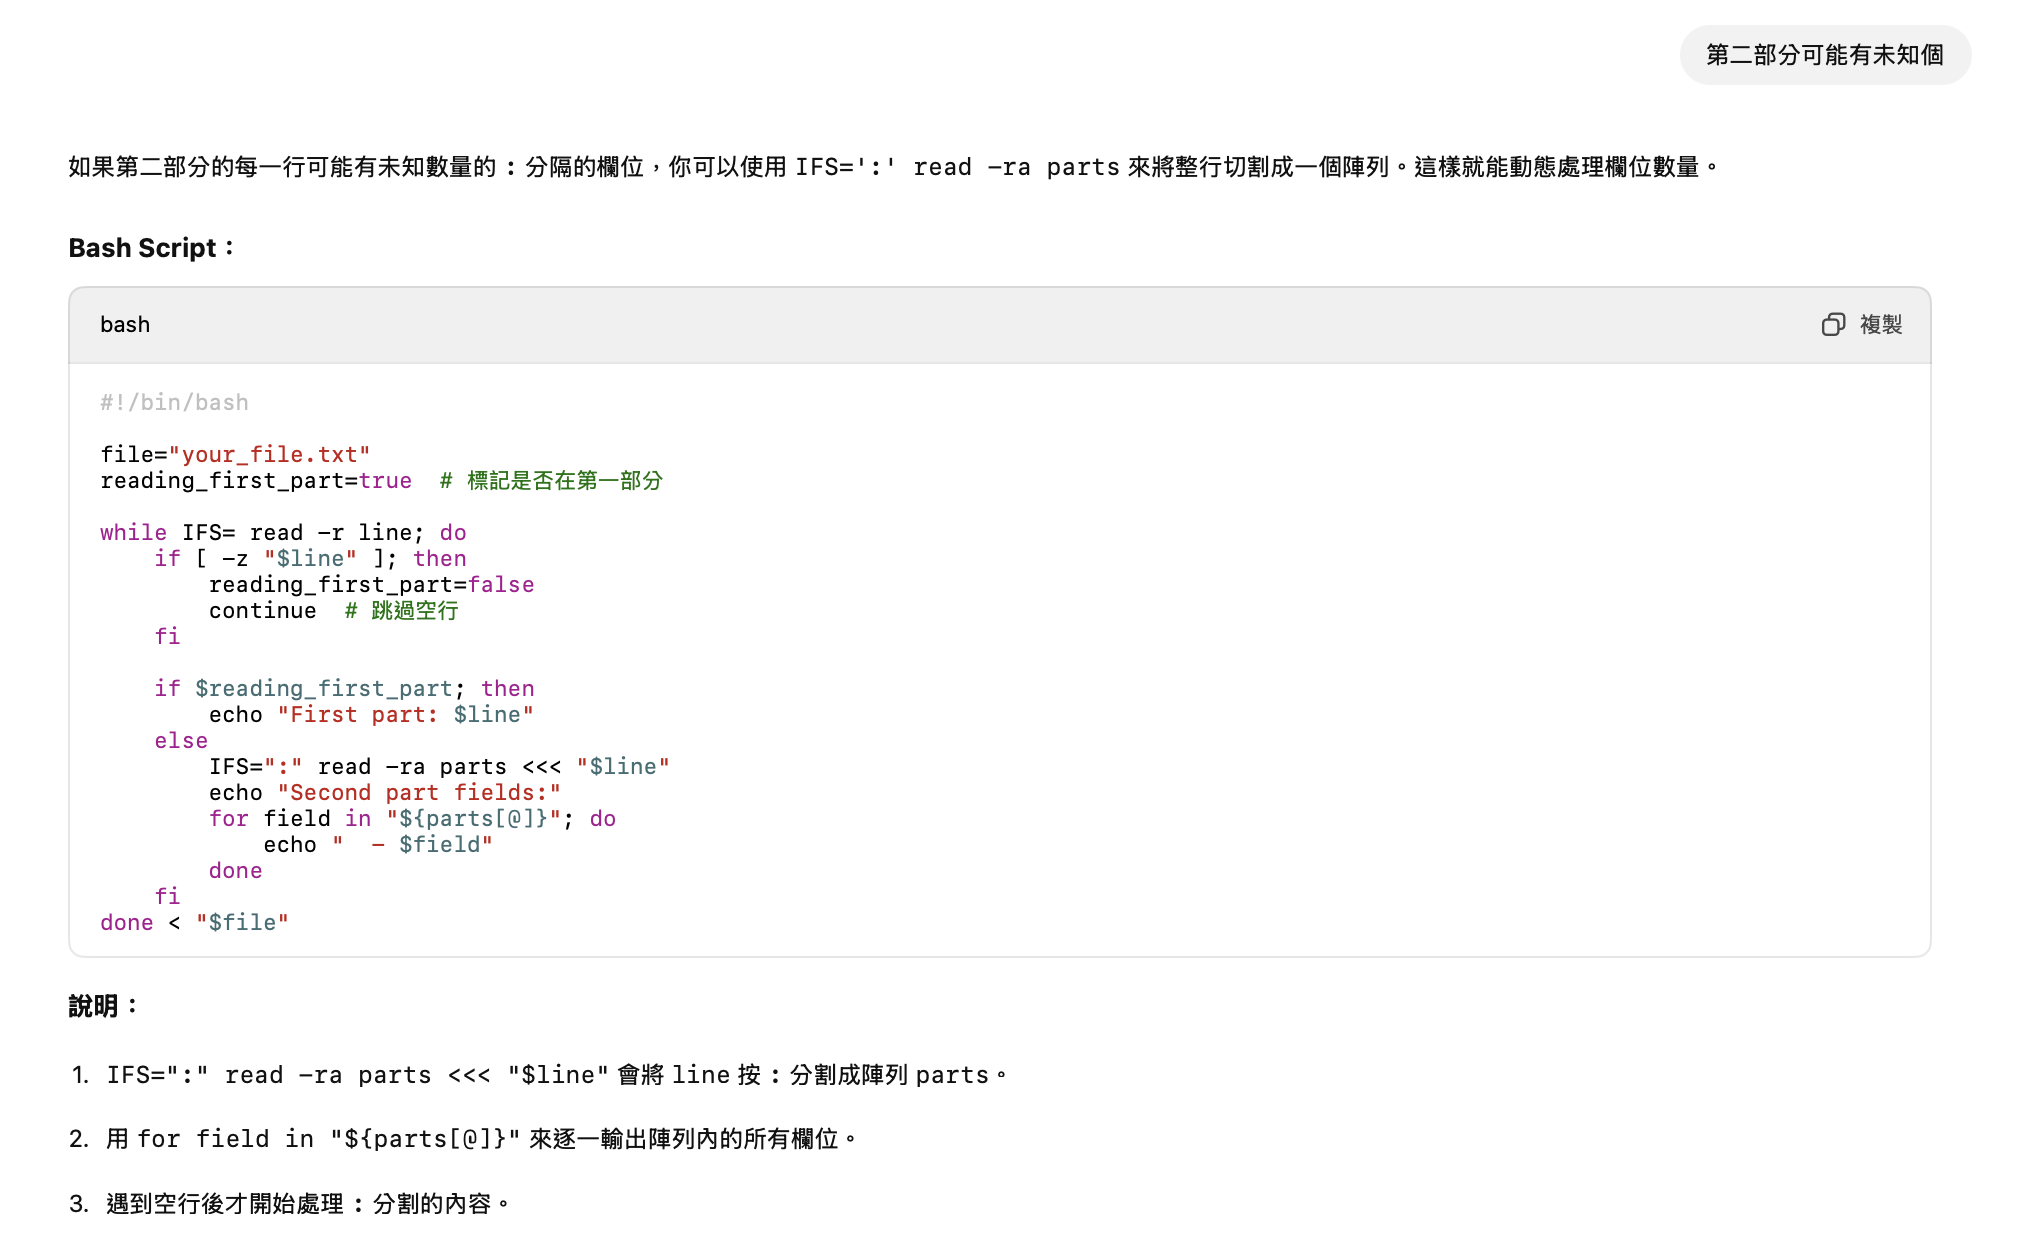
\includegraphics[width=\textwidth]{3-2.png}
  \end{figure}
\end{problem}

\clearpage
\begin{problem}{4.} \textbf{Verifying an Inclusion Proof}
  \begin{figure}[H]
    \centering
    
\includegraphics[width=\textwidth]{4-1.png}
    
\includegraphics[width=\textwidth]{4-2.png}
  \end{figure}
\end{problem}

% -----------------------------------------------------------
%    You don't have to mess with anything below this line.
% -----------------------------------------------------------

\end{document}
